\documentclass{article}
\usepackage{hyperref}
\usepackage{enumitem}
\usepackage{graphicx}
\usepackage{amsmath}

\begin{document}
\title{Technical Paper Proposal: \\ Placement Algorithms for Heterogenous FPGAs}
\author{Brian B Cheng \\ Department of Electrical and Computer Engineering}


\date{}
\maketitle

\section{Keywords}
\begin{itemize}
    \item FPGA, EDA, Synthesis, Placement, Routing, Parallel, Optimization
\end{itemize}


\section{Proposal}
A compiler takes a high-level program like a Java or Python file and assembles a corresponding machine code which is ready to be executed on a CPU.
In similar fashion, an Electronic Design Automation tool (EDA) takes a high-level description of a digital system written in Verilog or VHDL and produces a bitstream which is ready to be deployed to an FPGA.
In a superficial way, compilers and EDAs perform the same task for engineers but in different industries. 
One for software, the latter for hardware.

% Software compilers have become incredibly optimized over the decades and have allowed software engineers to be very productive. 
% The speed and user-friendliness that compilers offer allows engineers to push dozens, even hundreds of design cycles per day.
% Bugs and design changes can be patched and implemented into the program and recompiled in a matter of milliseconds to minutes. 
% Modern compilers are so refined that compilation can be regarded as where the "magic" happens in the software design cycle.
% Software engineers typically do not concern themselves with how their program gets compiled.
% Through multiple stages of lexing, parsing, and optimizations, the compiler takes the developer's program and produces working machine code.
% The developer can influence a few optimization flags if needed, but for the most part, the developer simply runs the default compiler command and is presented with the final product.
% All of this happens within milliseconds to seconds, even for large projects. 
% monotone, sentence length

Software compilers have evolved to become highly optimized, significantly boosting the productivity of software developers. 
The compilers are so robust that developers rarely need to worry about the correctness or efficiency of their machine code, and are so refined that it all happens in a matter of milliseconds to minutes, even for large projects. % break this up?
The speed of compilation enables rapid debugging and implementation of design changes and allows developers to iterate through dozens or even hundreds of design cycles per day.
Instead of tinkering around with assembly code, software engineers can comfortably focus on the high-level abstractions of their design. 

% Compilation, which takes mere milliseconds to minutes, enables rapid debugging and implementation of design changes. 
% The compilation process has become so streamlined that it can be considered the "magic" of the software development cycle. 
% They can influence a few optimization flags when needed, but for the most part, the developer simply runs the default compiler command.
% The compiler handles the lexing, parsing, and optimization automatically, with minimal input from the developer who typically relies on default settings unless specific optimization flags are needed. 
% Even for large-scale projects, this process is fast and efficient, allowing engineers to focus on higher-level design rather than low-level details.

The compilation stages mainly consists of lexing, parsing, and instruction optimization.
While these stages can be complex from a design standpoint, they are, mathematically, trivial.
The EDA stages are despairingly complex by comparison. 
First, the FPGA engineer creates and describes a digital design using a hardware description language (HDL) like Verilog or VHDL.     
Then the engineer submits the design entry to an EDA like Vivado or Quartus to perform three stages of automated design. 
These are: synthesis, placement, and routing. 
All three are NP-hard problems.

For even modest designs that utilize a small percentage of the available resources on the FPGA, the EDA will spend a minimum of a couple minutes synthesizing and implementing the design.
The EDA run time increases exponentially with the scale of the project. 
Projects that utilize 80\% or more of the FPGA's resources may run for hours, and for the high-end devices like Xilinx's Kintex FPGAs which have millions of logical elements, can run for days.
At high utilization, there is a possibility that the EDA cannot fit the design onto the device due to routing congestion even when it has enough logical elements to implement the design. 
The EDA might only reach this conclusion after attempting to fit the design for several hours. 

One of the most common complaints from new FPGA engineers, especially those coming from software development, is that the FPGA toolchains are overall slow and heavy.
This is because the problems that the EDA must solve are inherently complex.
Unlike in software development where an error in the program can be patched and recompiled in a matter of minutes, EDA runtimes lasting several hours means that an engineer can only go through a couple design cycles per day. 
An FPGA engineer must be very precise with their coding and practice thorough verification of their design before submitting it to the EDA.
This overall heightens the barrier of entry into FPGA development and contributes to a shortage of qualified FPGA engineers and a limitation of their productivity. 

This paper aims to study one particular pillar of this barrier: the placement stage. 
First, it will review prerequisite knowledge for placement algorithms. 
This includes graph theory to represent logical elements of a digital design and the wired connections between them, and a corresponding optimization problem with a cost function which we seek to minimize. 

In mathematics, a graph is usually modeled as \( G = (V, E) \), where \( V \) represents the set of vertices and \( E \) represents the set of edges between them.
A hypergraph is denoted as \( G_{H} = (V_{H}, E_{H}) \), where \( V_{H} \) represents the set of vertices, and \( E_{H} \) represents the set of hyperedges, which are edges that can connect more than two vertices.
Electronic circuits are typically represented as hypergraphs where % FINISH ME
In FPGA design, the graph is often modeled using a "netlist". A netlist is a graph \( G = (V, E) \), where \( V \) represents the components (e.g., logic blocks or gates), and \( E \) represents the connections or nets between them.

The vast majority of existing placers use the Half Perimeter Wire Length (HPWL) cost function or one of its various flavors - manhattan distance, euclidian distance, beta-regularized, etc..
The basic HPWL models the problem as the summation of the manhattan lengths of all nets in the netlist. 


\begin{equation}
    \text{HPWL} = \sum_{i=1}^{n} \left( \max_{j \in \text{net}_i} (x_j) - \min_{j \in \text{net}_i} (x_j) + \max_{j \in \text{net}_i} (y_j) - \min_{j \in \text{net}_i} (y_j) \right)
\end{equation}


Then, the paper will survey the current landscape of placement algorithms and strategies. 
This includes Simulated Annealing (SA), Analytical Placement (AP), 


\section{Abbreviations}
\begin{itemize}[label={--}, left=0.25cm]
    \item \textbf{FPGA}: Field Programmable Gate Array
    \item \textbf{VLSI}: Very Large Scale Integration
    \item \textbf{EDA}: Electronic Design Automation
    \item \textbf{VHSIC}: Very High Speed Integrated Circuits
    \item \textbf{HDL}: Hardware Description Language
    \item \textbf{VHDL}: VHSIC HDL
    \item \textbf{HLS}: High Level Synthesis: Generating synthesizable HDL from high-level software languages. A company might want to have a software engineer write C or C++ code and have a program translate it into synthesizable Verilog. This can can boost productivity and save the company the need to hire a hardware engineer.
    \item \textbf{IP}: Intellectual Property: In FPGA context, this means pre-built modules or subsystems like a hardened microprocessor or Ethernet controller. These are usually proprietary.
    \item \textbf{SoC}: System on Chip: An FPGA device (chip) that features hardened IP in addition to the programmable logic fabric.
    \item \textbf{PL-PS}: Programmable Logic - Processing System: A design that utilizes the on-chip hard microprocessor in conjunction with the programmable logic fabric.
    \item \textbf{EDIF}: Electronic Design Interchange Format
    \item \textbf{HPWL}: Half Perimeter Wire Length
\end{itemize}


\section{Ideas}
\begin{itemize}[label={\textbullet}, left=0.25cm]
    \item \textbf{FPGA}: Field Programmable Gate Array
    \begin{itemize}[label={--}, left=0.25cm]
        \item FPGA Vendors:
        \begin{itemize}[label={$\cdot$}, left=0.25cm]
            \item AMD-Xilinx ($\sim$50\% FPGA vendor market share)
            \item Intel-Altera ($\sim$35\% share)
            \item Lattice
            \item Microsemi
        \end{itemize}
    \end{itemize}

    \item \textbf{EDA}: Electronic Design Automation
    \begin{itemize}[label={--}, left=0.25cm]
        \item Proprietary software for FPGA and VLSI development:
        \begin{itemize}[label={$\cdot$}, left=0.25cm]
            \item Xilinx - Vivado (Design + Simulation) + Vitis (HLS + PL-PS codesign)
            \item Altera - Quartus (Design) + ModelSim (Simulation)
            \item Synopsis (VLSI)
            \item Cadence (VLSI)
        \end{itemize}
        \item Open source software for FPGA development:
        \begin{itemize}[label={$\cdot$}, left=0.25cm]
            \item \textbf{VTR}: Simulated Annealing placer for FPGAs. Popular among researchers who study placement techniques. 
                Commonly referred to as an "academic placer".
            \item \textbf{OSS-CAD}: a full-flow software suite that includes ABC synthesis, Yosys synthesis, Yosys nextpnr.
            \item \textbf{AMF-Placer}: Analytical Placer for FPGAs
            \item \textbf{RapidWright}: Semi-open source Java API that provides backend access to Xilinx Vivado EDA using design checkpoints.
            \item \textbf{RapidLayout}: Hard Block Placer for Systolic Arrays. Built with RapidWright.
            \item \textbf{RapidStream}: HLS Placer. Built with RapidWright.
            \item \textbf{DREAMPlace}: GPU-powered deep learning placement for VLSI.
            \item \textbf{DREAMPlaceFPGA}: DREAMPlace, adapted to FPGAs via the RapidWright API.
        \end{itemize}
    \end{itemize}
    
    \item \textbf{Synthesis}
    \begin{itemize}[label={--}, left=0.25cm]
        \item Takes a design written in a high-level HDL like VHDL or Verilog and "synthesizes" a \textbf{logical netlist} out of it. 
        \item The logical netlist is usually generated as an EDIF, JSON, or a low-level Verilog file. 
        \item The netlist describes the necessary basic elements of logic (BELs) and the wired connections between them that are necessary to implement the design.
    \end{itemize}

    \item \textbf{Placement}
    \begin{itemize}[label={--}, left=0.25cm]
        \item Takes the \textbf{logical netlist} and produces a \textbf{physical netlist}.
        \item For each BEL in the netlist, assign the BEL to a Cell, Site, and Tile on the physical FPGA device.
    \end{itemize}

    \item \textbf{Routing}
    \begin{itemize}[label={--}, left=0.25cm]
        \item Takes the \textbf{physical netlist} and maps the connections between BELs onto wires, interconnects, and switchboxes on the FPGA.
    \end{itemize}

\end{itemize}

\newpage
\begin{figure}
    \begin{center}
        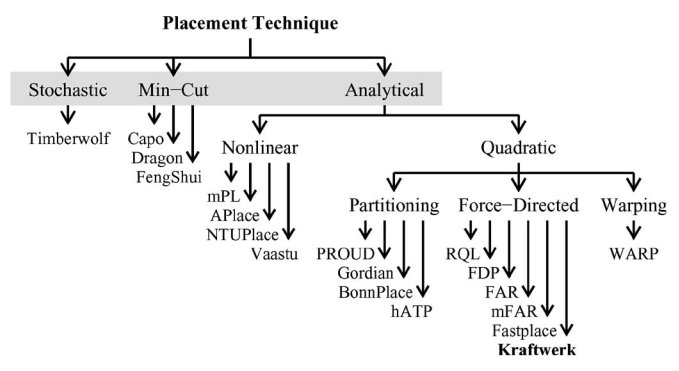
\includegraphics[width=0.75\textwidth]{figures/kraftwerk2.png}
    \end{center}
    \caption{Landscape of VLSI placement techniques (Spindler) \cite{kraftwerk2} }
    \label{fig:kraftwerk2}
\end{figure}
\begin{figure}
    \begin{center}
        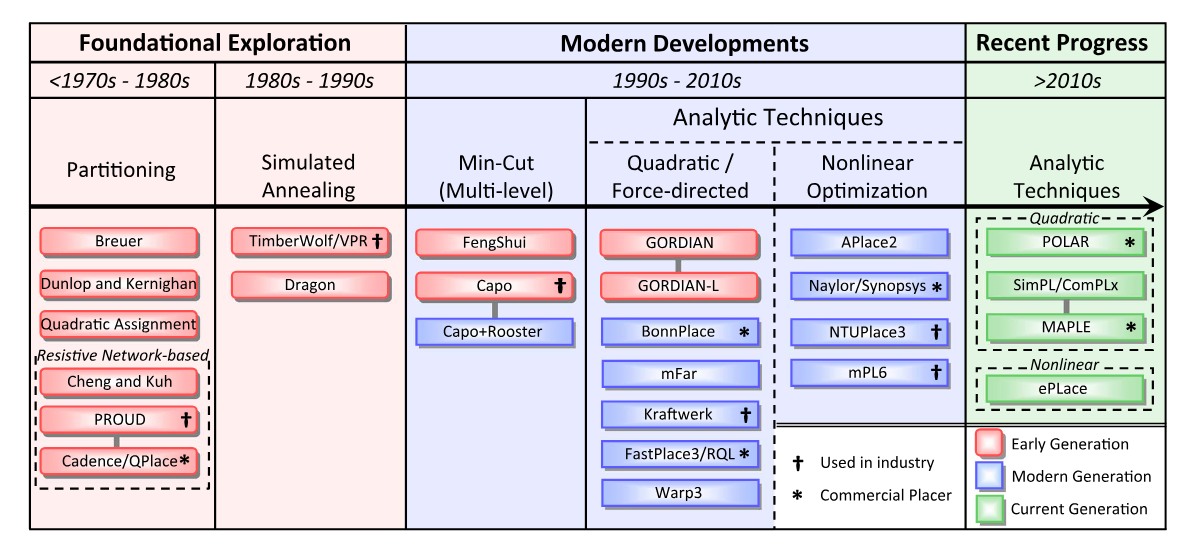
\includegraphics[width=0.95\textwidth]{figures/ProCha.png}
    \end{center}
    \caption{Historical timeline of VLSI placement techniques (Markov) \cite{ProCha} }
    \label{fig:ProCha}
\end{figure}

This is a citation for AMFPlacer. \cite{AMFPlacer}

\newpage
\bibliographystyle{ieeetr}
\nocite{*}
\bibliography{
    references/surveys,
    references/rapidwright,
    references/fpga_placement,
    references/vlsi_placement,
}
\end{document}


